\section{System Architecture}
The architecture of our proposed solution is shown in Figure \ref{sys-arch}.
In this section, we will give an overview of each of the blocks of the system.

\begin{figure}[h]
\label{sys-arch}
\centering
 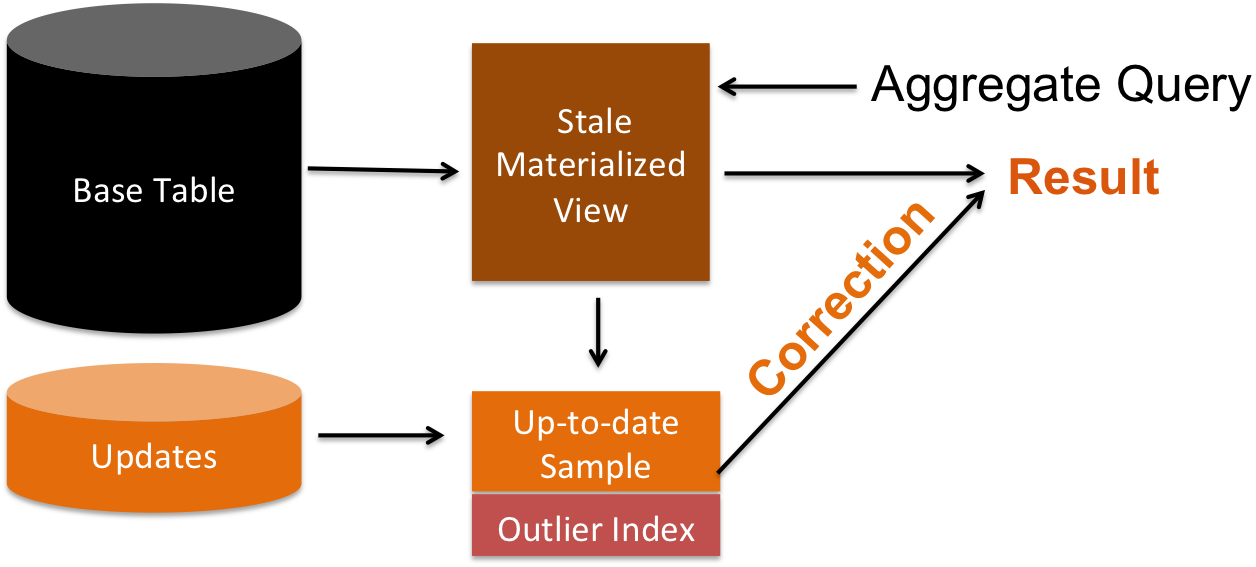
\includegraphics[width=\columnwidth]{figs/sys-arch.png}
 \caption{TODO}
\end{figure}

\subsection{Supported Materialized Views}

We will first introduce the taxonomy of materialized views
that can benefit from our approach. In particular, we provide example
situations when view maintenance can be costly. 

\subsubsection{Select-Project Views}

One type of view that we consider are views generated from Select-Project
expressions of the following form:

\begin{lstlisting}
SELECT [col1,col2,...] 
FROM table 
WHERE condition([col1,col2,...]) 
\end{lstlisting}
There are situations when such views are expensive to maintain. For
example, as often the case with activity logs, the base table may
contain semi-structured data that requires parsing or preprocessing
as a part of the view definition. Consider the following example,
a typical column in online activity logs is the User-Agent String
(Figure 1). When a user accesses a webpage the browser reports this
string to identify the browser type, operating system, and layout
engine. Suppose, we wanted to create a view of this dataset filtering
records to those that correspond users who used MacOS X and Safari.
This involves evaluating regular expression on the string to see if
it matches a criteria (eg. contains ``Mac OS X'' and contains ``Safari'').
Testing a complex regular expression will be far more expensive than
numerical comparisions or equality testing. In more extreme examples,
the columns may be serialized objects (eg. represented in JSON) which
need to be deserialized before evaluating a predicate.

%\begin{figure}
%\includegraphics[scale=0.3]{Documents/Research/sigmod15/Images/user-agent}

%\caption{User-Agent Activity Logs. <TODO>}
%\end{figure}



\subsubsection{Aggregation Views}

We also consider aggregation views of the following form:

\begin{lstlisting}
SELECT [f1(col1),f2(col2),...] 
FROM table 
WHERE condition([col1,col2,...]) 
GROUP BY [col1,col2,...]
\end{lstlisting}


While the same costs that Select-Project views can incur due to pre-process
apply as well, aggregation views pose additional challenges to incremental
view maintenance. Aggregation views can be costly to maintain when
the cardinality of the result is large; that is when there group by
clause is very selective. If the cardinality of the delta view is
large then it will be more costly to propagate this result with the existing
view. These costs increase in a distributed environment where a larger
delta view means that more data has to be communicated through a shuffle
operation. 


\subsubsection{Foreign-Key Join Views}

The third type of view we consider are Foreign-Key Join views:

\begin{lstlisting}
SELECT table1.[col1,col2,...], 
table2.[col1,col2,...]
FROM table1, table2 
WHERE table1.fk = table2.fk 
AND condition([col1,col2,...]) 
\end{lstlisting}


Such views are ubquitious in star schemas {[}?{]} and can be particularly
costly to maintain in distributed environments. In the example above,
suppose new recrods have been inserted into table1. Calculating the
delta view involves joining the new records with the entire table2.
While indexing is the prefered strategy to optimize such joins, many
distributed systems, such as Apache Spark, Cloudera Impala, and Apache
Tez, lack native support for join indices. To avoid scanning the entire
table, these systems rely on partitioned joins where records linked
by foreign keys are stored on the same partition. However, when these
join keys cross partition lines this operation can become increasingly
expensive.


\subsection{Reducing Maintenance Cost With Sampling}

We presented examples where these views can be expensive to maintain.
In this work, we address the question of whether we need to maintain
the entire view to answer aggregate queries on these views. Our proposed
solution is to sample the delta view $\Delta\textbf{V}$, and incrementally
maintain just a sample of $\textbf{V}_{T}$. For example, in our Select-Project
view example application, we would have to parse only a sample of
the inserted records. Similarly, for the Aggregation view, sampling
$\Delta\textbf{V}$ reduces the cardinality of the result and consequently
communication/merging costs. And finally, for the Join views, we would
only have to join a sample of the inserted records.


\subsection{Staleness and Correcting Staleness}

Given the three categories of views and the SUM, COUNT, AVG, and VAR
queries on these views, we can formalize the concept of staleness.
Let $\textbf{V}_{T}$ be the old view, and $\textbf{V}_{T}^{'}$ be
the up-to-date view. If $f$ is an aggregation function, then we call
the staleness error of the query $\epsilon$ if :
\[
f(\textbf{V}_{T}^{'})=f(\textbf{V}_{T})+\epsilon
\]
Since we already have the out-of-date view, we can easily compute
$f(\textbf{V}_{T})$. However, to get an up-to-date result, we need
an estimate of $\epsilon$. In {[}?{]}, the authors proposed an algorithm
called ``NormalizedSC'' which estimated the error term $\epsilon$
from a sample of the \emph{difference set}. The difference set is
defined in the following way: for a set of tuples $v_{i}^{'}\in\textbf{V}_{T}^{'}$
and $v_{j}\in\textbf{V}_{T}$ such that if tuple i is in both $\textbf{V}_{T}^{'}$
and $\textbf{V}_{T}$ then value $v_{i}^{'}-v_{i}$ is included and
if not the value $v_{i}'$ is included. If we denote this set as $\textbf{V}_{T}^{'}-\textbf{V}_{T}$$ $,
we can take a sample $S\subseteq\textbf{V}_{T}^{'}-\textbf{V}_{T}$,
and then we can apply the query to the sample $f(S)\approx\epsilon$.
The key result from {[}?{]} is that for a large enough sample size
$f(S)\sim N(\epsilon,\frac{\sigma_{diff}^{2}}{k})$ ; that is the
estimate is centered around the true value with variance proportional
to the differences and inversely proportional to the sample size.
With the an estimate $f(S)$, we can then correct a stale query $f(\textbf{V}_{T})-f(S)\approx f(\textbf{V}_{T}^{'})$
. This estimate is unbiased and probabilistically bounded.

We address a few new challenges in this work. First, NormalizedSC
was designed in the context of static tables and data errors that
can be modeled record transformations. In this context, it is clear
how to sample the set of differences. We can sample the dirty table
and then transform the records, and then take the differences. In
the following sections, we will describe how address the new challenges
of insertions. A further addition, is we consider the effects of outliers
on the estimate of NormalizedSC and characterize the optimality of
the NormalizedSC algorithm.

\subsection{Outlier Indexing}
We are often interested in records that outliers, 
which we define in this work as records with abnormally large attribute values.
Outliers and power-law distributions are a common property in web-scale datasets.
Often the queries of interest involve the outlier records, however sampling does 
have the potential to mask outliers in the updates.
If we have a small sampling ratio, more likely than not, outliers will be missed.

Therefore, we propose coupling sampling with outlier indexing. 
That is, we guarantee that records (or rows in the view derived from those records) 
with abnormally large attribute values are included in the sample.
What is particularly interesting is that these records give information about the distribution 
and can be used to reduce variance in our estimates.

\subsection{Relationship to SAQP}

Estimating the results of aggregate queries from samples has been
well studied in a field called Sample-based Approximate Query Processing
(SAQP). While the concept of estimating a correction from a sample
is similar to SAQP it differs in a few critical ways. Traditional
SAQP techniques apply their sampling directly to base tables and not
on views. The SAQP approach to this problem, would be to treat aggregate
queries on views as nested queries and then apply them to a sample
of the base data {[}?{]}. Another potential technique would be to
estimate the result directly from the maintained sample; a sort of
SAQP scheme on the sample of the view. We found that empricially estimating
a correction and leveraging an existing deterministic result lead
to lower variance results on real datasets (see Section ?). We analyze
the tradeoffs of these techniques in the following sections.